\section{Resultats}
\captionsetup[figure]{labelsep=space}
\subsection{Descripció de les dades}

Les dades obtingudes han estat les següents:

\begin{figure}[h!]
\centering
\begin{minipage}{0.45\linewidth}
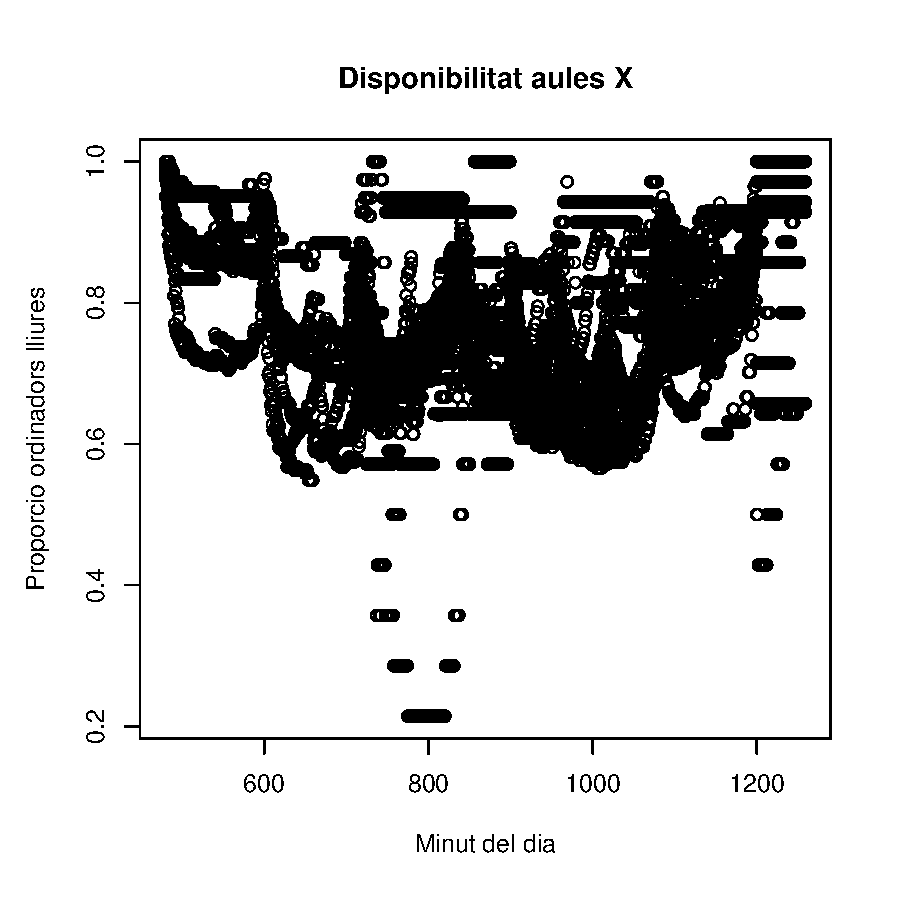
\includegraphics[width=1\linewidth]{./images/dades_X.eps}
\end{minipage}
\hfill
\begin{minipage}{0.45\linewidth}
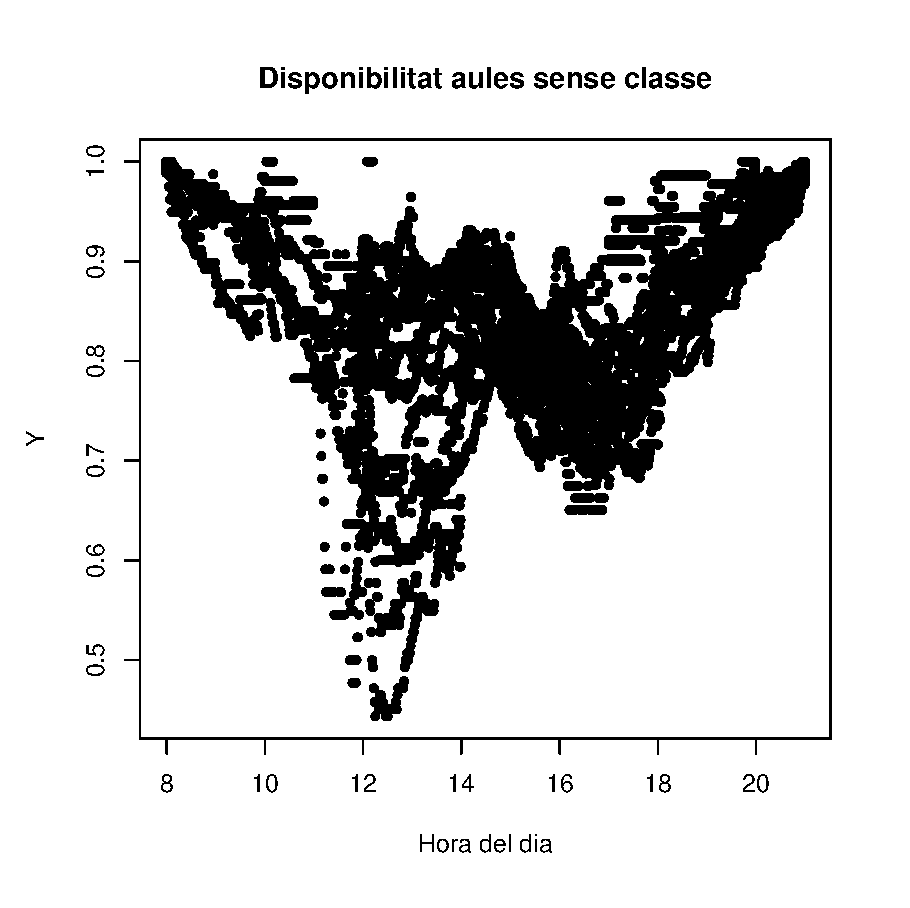
\includegraphics[width=1\linewidth]{./images/dades_Y.eps}
\end{minipage}
\end{figure}

Els dos gràfics són els reculls de dades per les aules amb classe i les aules sense classe. Cada punt és la proporció d'ordinadors lliures en una hora en concret.

\subsection{Comparació de la disponibilitat}


\begin{figure}[h!]
\begin{minipage}{0.5\linewidth}
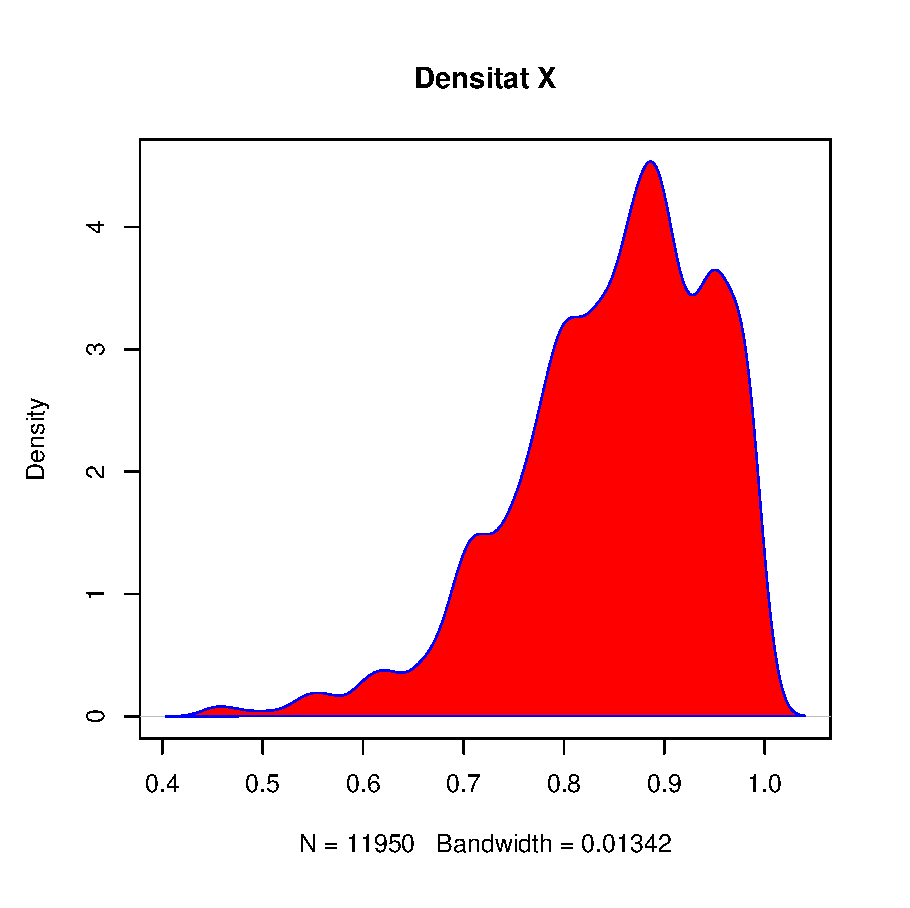
\includegraphics[width=1\linewidth]{./images/no_DENS.eps}
\caption{}
\end{minipage}
\hfill
\begin{minipage}{0.5\linewidth}
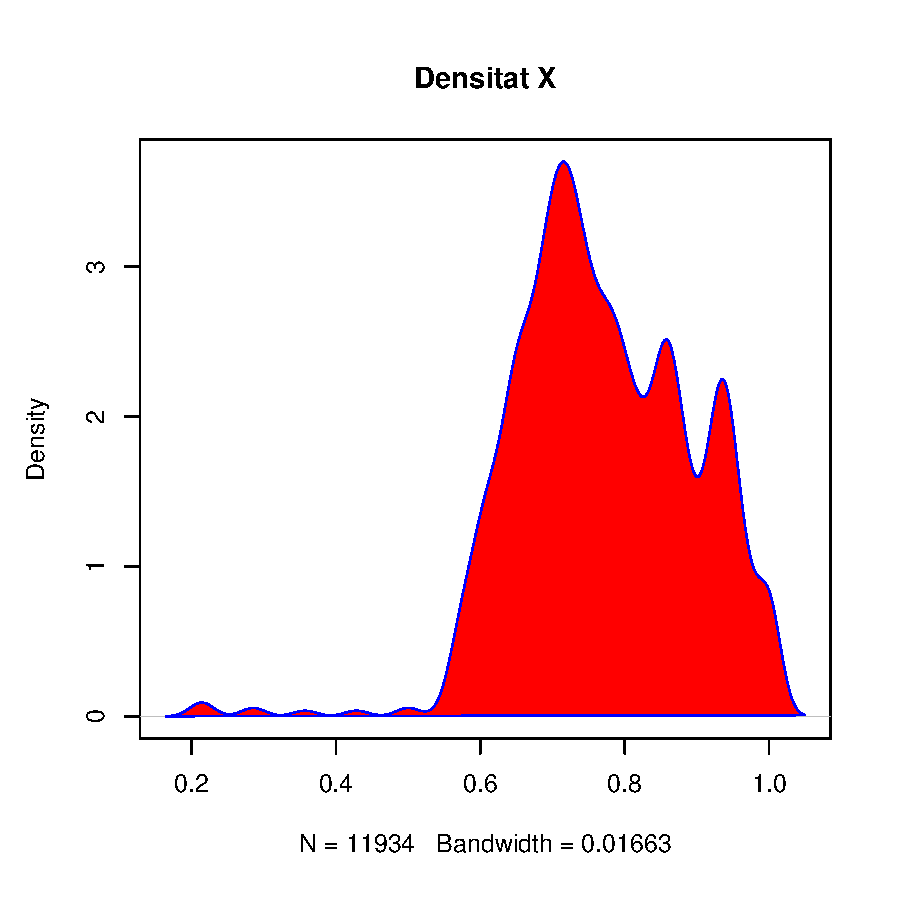
\includegraphics[width=1\linewidth]{./images/si_DENS.eps}
\caption{}
\end{minipage}
\end{figure}
Analitzant les dades obtingudes hem arribat als següents valors:
$$\bar{x} = 0.77083, s^2_x = 0.01459139, n_x = 11934$$
$$\bar{y} = 0.8503347, s^2_y = 0.009507904, n_y = 11950$$
I per tant:
$$\hat{z} = -55.96263$$


El valor de $\hat{z}$ és extremament petit. De fet, calculant el p-valor amb \emph{R} per aquesta $\hat{z}$ el resultat és 0. Per tant, queda clar que s'ha de rebutjar la hipòtesi nul·la. És més, degut a que $\hat{z}$ ha resultat ser negativa, podem afirmar que $\mu_Y > \mu_X$.